\documentclass{beamer}

\usepackage{graphicx}
\usepackage{textpos}
\usepackage{listings}
\usepackage{algorithm2e}
\usepackage{dijkstra}
\usepackage{tikz}
\usepackage{verbatim}

\usetikzlibrary{shapes.geometric}
\usetikzlibrary{arrows,shapes,trees}
\usetikzlibrary{calc,shapes.multipart,chains,arrows}
\usetikzlibrary{arrows,shapes}
\usetikzlibrary{arrows.meta, matrix, positioning}
\tikzset{
    queue element/.style={
        draw,very thin,rounded corners,
        fill=yellow!30,
        minimum width=1cm,minimum height=.5cm,
        font=\sffamily\footnotesize
    },
    >={[scale=0.8]Triangle},
    queue/.style={matrix of nodes,
        nodes in empty cells,
        nodes={queue element, anchor=center},
        fill=green!20,
        column sep=5mm,
        row sep=2mm,
    },
}

\usepackage[utf8]{inputenc}

\usetheme{Madrid}
\useoutertheme{miniframes} % Alternatively: miniframes, infolines, split

\usepackage{listings}
\lstset{language=Java,
    showspaces=false,
    showtabs=false,
    breaklines=true,
    showstringspaces=false,
    breakatwhitespace=true,
    commentstyle=\color{green},
    keywordstyle=\color{blue},
    stringstyle=\color{red},
    basicstyle=\footnotesize,
    moredelim=[is][\textcolor{grey}]{\%\%}{\%\%}
}

\definecolor{gray}{rgb}{0.4,0.4,0.4}
\definecolor{darkblue}{rgb}{0.0,0.0,0.6}
\definecolor{cyan}{rgb}{0.0,0.6,0.6}


% Setup the university's color pallette
\definecolor{UIUCorange}{RGB}{19, 41, 75} % UBC Blue (primary)
\definecolor{UIUCblue}{RGB}{232, 74, 39} % UBC Grey (secondary)


\setbeamercolor{palette primary}{bg=UIUCorange,fg=white}
\setbeamercolor{palette secondary}{bg=UIUCblue,fg=white}
\setbeamercolor{palette tertiary}{bg=UIUCblue,fg=white}
\setbeamercolor{palette quaternary}{bg=UIUCblue,fg=white}
\setbeamercolor{structure}{fg=UIUCorange} % itemize, enumerate, etc
\setbeamercolor{section in toc}{fg=UIUCblue} % TOC sections

\setbeamercolor{subsection in head/foot}{bg=UIUCorange,fg=UIUCblue}
\setbeamercolor{subsection in head/foot}{bg=UIUCorange,fg=UIUCblue}

\usepackage[utf8]{inputenc}


%Information to be included in the title page:
\title{\textbf{Dijkstra's Shortest Path\\ and\\ Prim's Minimum Spanning Tree}}
\author{\textbf{Author}}
\institute[\textbf{UIUC}]{\textbf{University of Illinois Urbana-Champaign}}
\date{\textbf{Date}}

\setbeamertemplate{title page}[default][colsep=-4bp,rounded=true]
\addtobeamertemplate{title page}{\vspace{3\baselineskip}}{}
\addtobeamertemplate{title page}{
    \begin{textblock*}{\paperwidth}(-1.0em, -1.2em)
        \includegraphics[width=\paperwidth, height=\paperheight]{imgs/uiuc.png}
    \end{textblock*} 
}{}

\begin{document}

\pgfdeclarelayer{background}
\pgfsetlayers{background,main}

\tikzstyle{vertex}=[circle,fill=black!25,minimum size=20pt,inner sep=0pt]
\tikzstyle{selected vertex} = [vertex, fill=orange!24]
\tikzstyle{edge} = [draw,thick,-]
\tikzstyle{weight} = [font=\small]
\tikzstyle{selected edge} = [draw,line width=5pt,-,blue!50]
\tikzstyle{ignored edge} = [draw,line width=5pt,-,black!20]


\frame{\titlepage}

\section{Priority Queues}

\begin{frame}[fragile]
    \frametitle{Queues vs Priority Queues}
    \begin{minipage}{0.47\textwidth}
        {\centering \textbf{Standard Queue}: Stores things in the offer they were enqueued.}
        \begin{figure}[H]
            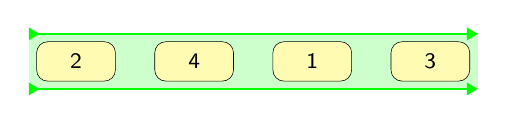
\begin{tikzpicture}
                \fill[green!20] (5.1,.35) rectangle (-.6,-.35);
                \draw[green,thick,>->] (-.6,.35) -- (5.1,.35);
                \draw[green,thick,>->] (-.6,-.35) -- (5.1,-.35);
                \foreach \i/\name in {0/2,1/4,2/1,3/3}
                \node[queue element] (\name) at (1.5*\i,0) {\name};
            \end{tikzpicture}
        \end{figure}
        \begin{lstlisting}
Queue<Integer> q = new ArrayDequeue<>();
q.offer(3); 
q.offer(1);
q.offer(4);
q.offer(2);
        \end{lstlisting}
        \vspace{1cm}
    \end{minipage}
    \hfill
    \vline
    \hfill
    \begin{minipage}{0.47\textwidth}
        \textbf{Priority Queue}: Reorders on insertion so the min or max value is always on top.\\
        \vspace{-0.2cm}
        \begin{figure}[H]
            \centering
            \scalebox{0.75}{
                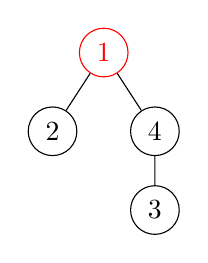
\begin{tikzpicture}[
    level distance = 1cm,
    level 1/.style = {sibling distance=1.3cm},
    level 2/.style = {sibling distance=1.0cm},
    level 3/.style = {sibling distance=0.8cm},
    every node/.style = {circle,draw},
    lbl/.style = {rectangle, draw=none, #1,% position
    font=\footnotesize}
    ]
    %
    \node (Root) [red] {1}
        child {node {2}
        }
        child { node {4}
            child { node {3} 
            }
            edge from parent node[lbl=left] {}
        };
\end{tikzpicture}



            }
        \end{figure}
        \vspace{-0.2cm}
        \begin{lstlisting}
Queue<Integer> pq = new PriorityQueue<>();
pq.offer(3); 
pq.offer(1);
pq.offer(4);
pq.offer(2);
        \end{lstlisting}
    \end{minipage}
\end{frame}

\section{Prim's MST}

\begin{frame}[fragile]
    \frametitle{Prim's Key Points}
    \begin{minipage}{0.49\textwidth}
        \centering
        \includegraphics[width=\textwidth]{./imgs/graph-1.png}
    \end{minipage}
    \hfill
    \begin{minipage}{0.49\textwidth}
        \centering
        \resizebox{0.80\textwidth}{!}{
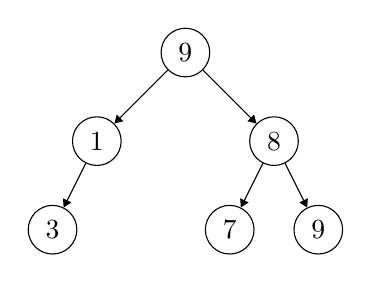
\begin{tikzpicture}[level distance=1.5cm,
    level 1/.style={sibling distance=3cm},
    level 2/.style={sibling distance=1.5cm},
    every node/.style = {minimum width = 1.75em, draw, circle},
    scale=0.75
    ]
    \node {9}
        child {node[] {1}
            child {node[] {3} edge from parent[->]}
            child {edge from parent[draw = none]}
            edge from parent[->]
        }
        child {node[] {8} 
            child {node[]{7} edge from parent[->]}
            child {node[]{9} 
                edge from parent[->]
            }
            edge from parent[->]
        };
\end{tikzpicture}
}

    \end{minipage}
    \begin{itemize}
        \item \textbf{Purpose:} For an weighted undirected graph, Prim's MST finds a subgraph (tree) that meets the following condition:
            \begin{enumerate}
                \item All vertices are reachable.
                \item The sum of the edges in the graph are minimized.
            \end{enumerate}
    \end{itemize}
\end{frame}

\begin{frame}[fragile]
    \frametitle{Prim's Key Points}
    \begin{minipage}{0.49\textwidth}
        \centering
        \includegraphics[width=\textwidth]{./imgs/graph-1.png}
    \end{minipage}
    \hfill
    \begin{minipage}{0.49\textwidth}
        \centering
        \resizebox{0.80\textwidth}{!}{
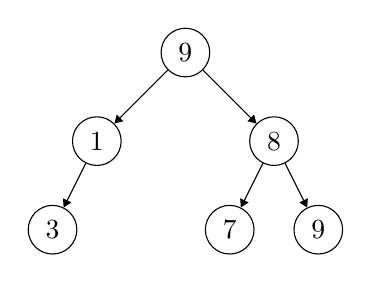
\begin{tikzpicture}[level distance=1.5cm,
    level 1/.style={sibling distance=3cm},
    level 2/.style={sibling distance=1.5cm},
    every node/.style = {minimum width = 1.75em, draw, circle},
    scale=0.75
    ]
    \node {9}
        child {node[] {1}
            child {node[] {3} edge from parent[->]}
            child {edge from parent[draw = none]}
            edge from parent[->]
        }
        child {node[] {8} 
            child {node[]{7} edge from parent[->]}
            child {node[]{9} 
                edge from parent[->]
            }
            edge from parent[->]
        };
\end{tikzpicture}
}

    \end{minipage}
    ~\\
    \begin{itemize}
        \item \textbf{Greedy Algorithm: } A algorithm that uses of making the optimal decision at each individual step such that the sum of these locale ally optimal steps leads to a globally optimal solution.
        \item \textbf{Prim's Greedy Heuristic: } Visit a reachable vertex with the smallest distance between it and it's parent at each step.
    \end{itemize}
\end{frame}


\section{Prim's - Walkthrough}

\begin{frame}[fragile]
    \frametitle{The Algorithm - Setup (Steps 1 \& 2)}
    \centering
    \begin{minipage}{0.69\textwidth}
        \includegraphics[width=0.69\textwidth]{./imgs/prims-1-2.png}
    \end{minipage}
    \hspace{-3cm}
    \begin{minipage}{0.49\textwidth}
        \small
        \begin{itemize}
            \item \textbf{Step 1:} For each vertex, initialize the parents and the distance to that parent to be null and infinity (\texttt{Integer.MAX\_VALUE}), respectively .
            \item \textbf{Step 2:} The source distance to parent to be 0, make a priority queue, and place that vertex in it.
                \begin{itemize}
                    \item After doing this, what will be the first entry in the PQ? Why?
                \end{itemize}
        \end{itemize}
    \end{minipage}
\end{frame}

\begin{frame}[fragile]
    \frametitle{The Algorithm - Finding the MST (Steps 3-5)}
    \centering
    \begin{minipage}{0.69\textwidth}
        \includegraphics[width=0.69\textwidth]{./imgs/prims-3-4-5.png}
    \end{minipage}
    \hspace{-3cm}
    \begin{minipage}{0.49\textwidth}
        \small
        \begin{itemize}
            \item \textbf{Step 3:} While there are still nodes unvisited, get the node with the minimum distance to it's parent (i.e., a node that's already been visited)
            \item \textbf{Step 4:} For each vertex adjacent to $U$, check if hasn't been visited (still in PQ) and if the weight from it to the vertex we're visiting is less than it's previous weight.
            \item \textbf{Step 5:} If it is, update the parent and the weight to that parent.
        \end{itemize}
    \end{minipage}
\end{frame}


\begin{frame}[fragile]
    \frametitle{Prim's - Iteration 1}
    \centering
    \begin{table}[]
        \begin{tabular}{|l|l|l|l|l|l|l|l|}
            \hline
            Vertex   & D        & A        & B        & C        & E        & F        & G        \\ \hline
            Parent   & -        & -        & -        & -        & -        & -        & -        \\ \hline
            Distance & 0 & $\infty$ & $\infty$ & $\infty$ & $\infty$ & $\infty$ & $\infty$ \\ \hline
        \end{tabular}
    \end{table}
    \includegraphics[width=0.45\textwidth]{./imgs/prims_walkthrough/prims1.png}
    \vspace{-0.2cm}
    \begin{table}[]
        \begin{tabular}{|l|l|l|l|l|l|l|l|}
            \hline
            Vertex   &  A        & B        & C        & E        & F        & G        \\ \hline
            Parent   &           &          &          &          &          &          \\ \hline
            Distance &  $      $ & $      $ & $      $ & $      $ & $      $ & $      $ \\ \hline
        \end{tabular}
    \end{table}
\end{frame}

\begin{frame}[fragile]
    \title{Prim's - Iteration 2}
    \centering
    \begin{table}[]
        \begin{tabular}{|l|l|l|l|l|l|l|}
            \hline
            Vertex   & A & F & B & E  & C        & G        \\ \hline
            Parent   & D & D & D & D  & -        & -        \\ \hline
            Distance & 5 & 6 & 9 & 15 & $\infty$ & $\infty$ \\ \hline
        \end{tabular}
    \end{table}
    \includegraphics[width=0.45\textwidth]{./imgs/prims_walkthrough/2.png}
    \begin{table}[]
        \begin{tabular}{|l|l|l|l|l|l|}
            \hline
            Vertex   & F & B & E  & C        & G        \\ \hline
            Parent   &  &  &      &          &         \\ \hline
            Distance &  &  &      &          &  \\ \hline
        \end{tabular}
    \end{table}

\end{frame}

\begin{frame}[fragile]
    \title{Prim's - Iteration 3}
    \centering
    \begin{table}[]
        \begin{tabular}{|l|l|l|l|l|l|}
            \hline
            Vertex   & F & B & E  & C        & G        \\ \hline
            Parent   & D & A & D  & -        & -        \\ \hline
            Distance & 6 & 7 & 15 & $\infty$ & $\infty$ \\ \hline
        \end{tabular}
    \end{table}
    \includegraphics[width=0.49\textwidth]{./imgs/prims_walkthrough/prims3.png}
    \begin{table}[]
        \begin{tabular}{|l|l|l|l|l|}
            \hline
            Vertex   & B & E & G  & C        \\ \hline
            Parent   &  &  &   &         \\ \hline
            Distance &  &  &  & \\ \hline
        \end{tabular}
    \end{table}

\end{frame}

\begin{frame}[fragile]
    \title{Prim's - Iteration 4}
    \centering
    \begin{table}[]
        \begin{tabular}{|l|l|l|l|l|}
            \hline
            Vertex   & B & E & G  & C        \\ \hline
            Parent   & A & F & F  & -        \\ \hline
            Distance & 7 & 8 & 11 & $\infty$ \\ \hline
        \end{tabular}
    \end{table}
    \includegraphics[width=0.49\textwidth]{./imgs/prims_walkthrough/prims4.png}
    \begin{table}[]
        \begin{tabular}{|l|l|l|l|}
            \hline
            Vertex   & E & C & G  \\ \hline
            Parent   &  &  &   \\ \hline
            Distance &  &  &  \\ \hline
        \end{tabular}
    \end{table}

\end{frame}

\begin{frame}[fragile]
    \title{Prim's - Iteration 5}
    \centering
    \begin{table}[]
        \begin{tabular}{|l|l|l|l|}
            \hline
            Vertex   & E & C & G  \\ \hline
            Parent   & B & B & F  \\ \hline
            Distance & 7 & 8 & 11 \\ \hline
        \end{tabular}
    \end{table}
    \includegraphics[width=0.49\textwidth]{./imgs/prims_walkthrough/prims5.png}
    \begin{table}[]
        \begin{tabular}{|l|l|l|}
            \hline
            Vertex   & C & G \\ \hline
            Parent   &  &  \\ \hline
            Distance &  &  \\ \hline
        \end{tabular}
    \end{table}

\end{frame}

\begin{frame}[fragile]
    \title{Prim's - Iteration 6}
    \centering
    \begin{table}[]
        \begin{tabular}{|l|l|l|}
            \hline
            Vertex   & C & G \\ \hline
            Parent   & E & E \\ \hline
            Distance & 5 & 9 \\ \hline
        \end{tabular}
    \end{table}
    \includegraphics[width=0.49\textwidth]{./imgs/prims_walkthrough/prims6.png}
    \begin{table}[]
        \begin{tabular}{|l|l|}
            \hline
            Vertex   & G \\ \hline
            Parent   &  \\ \hline
            Distance &  \\ \hline
        \end{tabular}
    \end{table}

\end{frame}

\begin{frame}[fragile]
    \title{Prim's - Iteration 7}
    \centering
    \begin{table}[]
        \begin{tabular}{|l|l|}
            \hline
            Vertex   & G \\ \hline
            Parent   & E \\ \hline
            Distance & 9 \\ \hline
        \end{tabular}
    \end{table}
    \includegraphics[width=0.49\textwidth]{./imgs/prims_walkthrough/prims7.png}

\end{frame}

\begin{frame}[fragile]
    \frametitle{Outputting the MST}
    \centering
    \begin{itemize}
        \item After the algorithm has run, the edges that make up the MST will be stored in the vertex-parent pairs. To output the MST, iterate over the vertices and print out those pairs.
        \item We could also keep track as we traverse (like BST).
    \end{itemize}
\end{frame}

\section{Dijkstra's SP}

\begin{frame}[fragile]
    \frametitle{Dijkstra's Key Points}
    \begin{figure}[H]
        \includegraphics[width=0.49\textwidth]{./imgs/dijkstra-from-d.png}
    \end{figure}
    \begin{itemize}
        \item \textbf{Goal:} Find the shortest path from a source vertex to every vertex in the graph.
        \item \textbf{Dijkstra's Greedy Heuristic:} At each step, visit the vertex that has the minimum distance \textit{from our source}.
    \end{itemize}
\end{frame}

\begin{frame}[fragile]
	\frametitle{Prim's vs Dijkstra's }
    \begin{minipage}{0.45\textwidth}\
        \vfill
        \footnotesize
        \noindent\textbf{Prim's MST:}\\
        \tiny
        \begin{algorithm}[H]
            \DontPrintSemicolon
            \While{PQ $\neq \emptyset$}{
                u $\gets$ PQ.getMin()\;
                \For{e $\in$ G.Adj[u]}{
                    \If{e.dest $\in$ PQ AND e.weight $<$ v.dist}{
                        v.parent $\gets$ u\;
                        v.dist $\gets$ e.weight\;
                        PQ.reprioritize(v);
                    }
                }
            }
        \end{algorithm}
        \begin{itemize}
            \item Selecting the vertex that has and edge accessing it which has the minimum distance overall.
            \item Updating the distance associated with that vertex if we find another edge that accesses it that has a lower weight.
        \end{itemize}
    \end{minipage}
    \hfill
    \vline
    \hfill
    \begin{minipage}{0.49\textwidth}
        \footnotesize
        \vfill
        \noindent\textbf{Dijkstra's SP:}\\
        \tiny
        \begin{algorithm}[H]
            \DontPrintSemicolon
            \While{PQ $\neq \emptyset$}{
                u $\gets$ PQ.getMin()\;
                \For{v $\in$ G.Adj[u]}{
                    PathWeight $\gets$ u.Distance + Weight(u, v)\;
                    \If{v $\in$ PQ AND pathWeight $<$ v.Distance}{
                        v.parent $\gets$ u\;
                        v.distance $\gets$ PathWeight\;
                        PQ.reprioritize(v);
                    }
                }
            }
        \end{algorithm}
        \begin{itemize}
            \item Selecting the vertex that has the minimum distance \textit{from our source}.
            \item We are checking to see if this vertex provides a shorter path
                to any of it's adjacent notes and updating their parent and
                distance if so.
        \end{itemize}
    \end{minipage}
\end{frame}



\section{Dijkstra's SP - Walkthrough}

\begin{frame}[fragile]
    \centering
    \begin{table}[]
        \begin{tabular}{|l|l|l|l|l|l|l|l|}
            \hline
            Vertex   & D & A        & B        & C        & E        & F        & G        \\ \hline
            Parent   & - & -        & -        & -        & -        & -        & -        \\ \hline
            Distance & 0 & $\infty$ & $\infty$ & $\infty$ & $\infty$ & $\infty$ & $\infty$ \\ \hline
        \end{tabular}
    \end{table}
    \includegraphics[width=0.45\textwidth]{./imgs/dijkstra_walkthrough/dijkstra-1.png}
    \begin{table}[]
        \begin{tabular}{|l|l|l|l|l|l|l|}
            \hline
            Vertex   & A & F & B & E  & C        & G        \\ \hline
            Parent   &  &  &  &   &         &         \\ \hline
            Distance &  &  &  &   &  &  \\ \hline
        \end{tabular}
    \end{table}
\end{frame}

\begin{frame}[fragile]
    \centering
    \begin{table}[]
        \begin{tabular}{|l|l|l|l|l|l|l|}
            \hline
            Vertex   & A & F & B & E  & C        & G        \\ \hline
            Parent   & D & D & D & D  & -        & -        \\ \hline
            Distance & 5 & 6 & 9 & 15 & $\infty$ & $\infty$ \\ \hline
        \end{tabular}
    \end{table}
    \includegraphics[width=0.45\textwidth]{./imgs/dijkstra_walkthrough/dijkstra-2.png}
    \begin{table}[]
        \begin{tabular}{|l|l|l|l|l|l|}
            \hline
            Vertex   & F & B & E  & C        & G        \\ \hline
            Parent   &  &  &     &         &         \\ \hline
            Distance &  &  &  &  & \\ \hline
        \end{tabular}
    \end{table}
\end{frame}

\begin{frame}[fragile]
    \centering
    \begin{table}[]
        \begin{tabular}{|l|l|l|l|l|l|}
            \hline
            Vertex   & F & B & E  & C        & G        \\ \hline
            Parent   & D & D & D  & -        & -        \\ \hline
            Distance & 6 & 9 & 15 & $\infty$ & $\infty$ \\ \hline
        \end{tabular}
    \end{table}
    \includegraphics[width=0.45\textwidth]{./imgs/dijkstra_walkthrough/dijkstra-3.png}
    \begin{table}[]
        \begin{tabular}{|l|l|l|l|l|}
            \hline
            Vertex   & B & E  & C  & G  \\ \hline
            Parent   &  &   &   &   \\ \hline
            Distance &  &   &   &  \\ \hline
        \end{tabular}
    \end{table}
\end{frame}

\begin{frame}[fragile]
    \centering
    \begin{table}[]
        \begin{tabular}{|l|l|l|l|l|}
            \hline
            Vertex   & B & E  & G  & C  \\ \hline
            Parent   & D & F  & F  & -  \\ \hline
            Distance & 9 & 14 & 17 & $\infty$ \\ \hline
        \end{tabular}
    \end{table}
    \includegraphics[width=0.45\textwidth]{./imgs/dijkstra_walkthrough/dijkstra-4.png}
    \begin{table}[]
        \begin{tabular}{|l|l|l|l|}
            \hline
            Vertex   & E  & G  & C  \\ \hline
            Parent   &    &    &   \\ \hline
            Distance &    &    &  \\ \hline
        \end{tabular}
    \end{table}
\end{frame}

\begin{frame}[fragile]
    \centering
    \begin{table}[]
        \begin{tabular}{|l|l|l|l|}
            \hline
            Vertex   & E  & G  & C  \\ \hline
            Parent   & F  & F  & B  \\ \hline
            Distance & 14 & 17 & 17 \\ \hline
        \end{tabular}
    \end{table}
    \includegraphics[width=0.45\textwidth]{./imgs/dijkstra_walkthrough/dijkstra-5.png}
    \begin{table}[]
        \begin{tabular}{|l|l|l|}
            \hline
            Vertex   & C  & G  \\ \hline
            Parent   &   &   \\ \hline
            Distance &   &  \\ \hline
        \end{tabular}
    \end{table}
\end{frame}

\begin{frame}[fragile]
    \centering
    \begin{table}[]
        \begin{tabular}{|l|l|l|}
            \hline
            Vertex   & C  & G  \\ \hline
            Parent   & B  & F  \\ \hline
            Distance & 17 & 17 \\ \hline
        \end{tabular}
    \end{table}
    \includegraphics[width=0.45\textwidth]{./imgs/dijkstra_walkthrough/dijkstra-7.png}
    \begin{table}[]
        \begin{tabular}{|l|l|l|}
            \hline
            Vertex   &  G  \\ \hline
            Parent   &    \\ \hline
            Distance &   \\ \hline
        \end{tabular}
    \end{table}
\end{frame}

\begin{frame}[fragile]
    \centering

    \begin{table}[]
        \begin{tabular}{|l|l|l|}
            \hline
            Vertex   &  G  \\ \hline
            Parent   &  F  \\ \hline
            Distance &  17 \\ \hline
        \end{tabular}
    \end{table}

    \includegraphics[width=0.45\textwidth]{./imgs/dijkstra_walkthrough/dijkstra-8.png}
    \\
    \textbf{Done!}

\end{frame}

\begin{frame}[fragile]
    \centering

    \includegraphics[width=0.45\textwidth]{./imgs/dijkstra_walkthrough/dijkstra-2.png}

\end{frame}

\begin{frame}[fragile]
    \frametitle{Outputting the Shortest path from Source to Dest}
    \centering
    \includegraphics[width=0.45\textwidth]{./imgs/dijkstra_walkthrough/dijkstra-8.png}
    \begin{itemize}
        \item Start at the destination you're wanting to visit.
        \item Work your way backwards keeping track of each step.
        \item Stop once you've found the source.
    \end{itemize}
\end{frame}

\section{Java PQ}
\begin{frame}[fragile]
    \frametitle{How do we do this in Java? Priority Queues + HashMap}
    \begin{lstlisting}
Map<E, E> parents = new HashMap<>();
Map<E, Integer> dists = new HashMap<>();

// We create a priority queue that orders things
// based on the value they're associated with in
// the hashmap.
Queue<E> pq = new PriorityQueue<E>(
    //tells the PQ to dists.get(vertex) to compare each edge
    Comparator.comparing(dists) 
);
    \end{lstlisting}
    \begin{itemize}
        \item Like BFS and DFS we will use HashMaps to keep track of values associated with vertices:
            \begin{itemize}
                \item \lstinline|parents| keeps track of each vertex's parent.
                \item \lstinline|dists| keeps track of the distance to that vertex.
                \item \lstinline|pq| keeps track of: 1) what vertexes are left and 2) orders them based on their distance in \lstinline|dists|.
            \end{itemize}
        \item To ``reprioritize'' the priority queue, we need to remove and readd a vertex every time we update it's distance.
    \end{itemize}
\end{frame}



\end{document}
